\documentclass[crop,tikz]{standalone}

\usepackage{tikz}
\usepackage{pgfplots}
\usepackage[utf8]{inputenc}

\newcommand{\cmpW}{7cm}
\newcommand{\cmpH}{4.0cm}
\newcommand{\legX}{0.45}
\newcommand{\legY}{-0.30}
\newcommand{\dtree}[1]{$#1$-d~tree}
\newcommand{\kdtree}{\dtree{k}}

\begin{document}
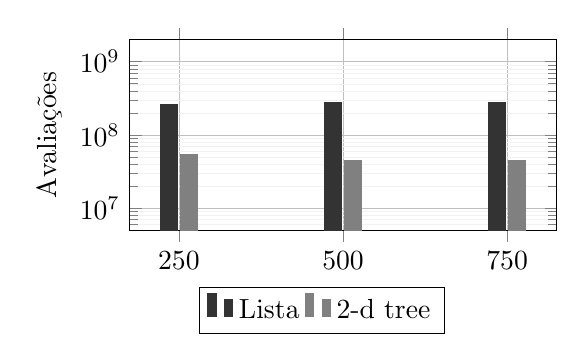
\begin{tikzpicture}
\begin{axis}[
	x tick label style={ /pgf/number format/1000 sep=},
	xtick=data,
	ymin=10000000,
	ymax=1000000000,
	width=\cmpW, height=\cmpH,
	ylabel=Avaliações,
	ymode=log,
	grid = both,
	grid style={line width=.1pt, draw=gray!10},
	major grid style={line width=.2pt,draw=gray!50},
	%xlabel=Number of items (n),
	enlargelimits=0.15,
	legend style={at={(\legX,\legY)},
		anchor=north,legend columns=-1},
	ybar=1.2pt,% configures `bar shift'
	bar width=6pt,
	point meta=y *10^-9, % the displayed number
	cycle list = {black!80,black!50,black!30}
]

\addplot+[fill, text=black]
  coordinates {
    ( 250,262753176)
    ( 500,275497548)
    ( 750,276160499)
  };
  
\addplot+[fill, text=black]
  coordinates {
    ( 250,53541348)
    ( 500,45332656)
    ( 750,45113125)
  };

\legend {Lista,\dtree{2}}
\end{axis}
\end{tikzpicture}

\end{document}
